\documentclass[tikz,border=4pt]{standalone}
% Paleta y fuentes compartidas por el libro y las figuras (única fuente de verdad).
\RequirePackage{xcolor}
\definecolor{oxido}{HTML}{B7410E}
\definecolor{cobre}{HTML}{D27D2D}
\definecolor{carbon}{HTML}{2B2B2B}
\definecolor{azul}{HTML}{1F5F8B}
\definecolor{arena}{HTML}{F4EDE4}

\usepackage{fontspec}
\setsansfont{FiraSans}[Extension=.otf,UprightFont=*-Regular,BoldFont=*-SemiBold,ItalicFont=*-Italic,BoldItalicFont=*-SemiBoldItalic]
\setmonofont{FiraMono}[Extension=.otf,UprightFont=*-Regular,BoldFont=*-Medium,Scale=0.95]
\usetikzlibrary{positioning,arrows.meta,calc,decorations.pathreplacing}
\begin{document}
\sffamily\small
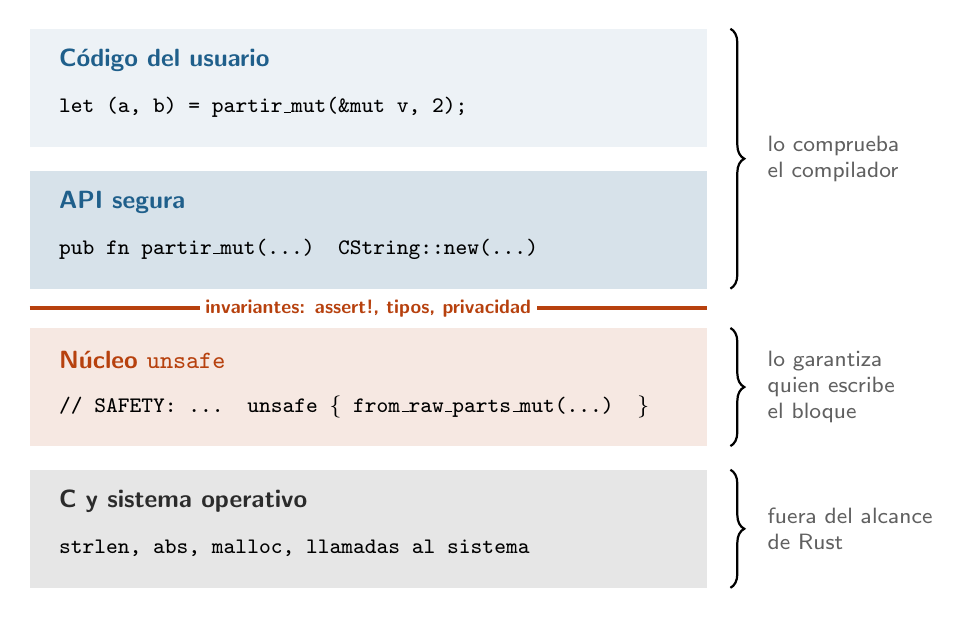
\begin{tikzpicture}[>={Stealth[length=2.2mm]},
  titulo/.style={font=\sffamily\small\bfseries,anchor=west},
  cod/.style={font=\ttfamily\footnotesize,anchor=west},
  nota/.style={font=\sffamily\footnotesize,text=carbon!75,anchor=west,align=left},
  llave/.style={decorate,decoration={brace,amplitude=5pt},line width=0.8pt}]
  % Capa 1: código del usuario
  \fill[azul!8] (0,0) rectangle (8.6,-1.5);
  \node[titulo,text=azul] at (0.25,-0.4) {Código del usuario};
  \node[cod] at (0.25,-1.0) {let (a, b) = partir\_mut(\&mut v, 2);};
  % Capa 2: API segura
  \fill[azul!18] (0,-1.8) rectangle (8.6,-3.3);
  \node[titulo,text=azul] at (0.25,-2.2) {API segura};
  \node[cod] at (0.25,-2.8) {pub fn partir\_mut(...)\quad CString::new(...)};
  % Frontera de invariantes
  \draw[oxido,line width=1.4pt] (0,-3.55) -- (8.6,-3.55);
  \node[font=\sffamily\scriptsize\bfseries,text=oxido,fill=white,inner sep=2pt]
    at (4.3,-3.55) {invariantes: assert!, tipos, privacidad};
  % Capa 3: núcleo unsafe
  \fill[oxido!12] (0,-3.8) rectangle (8.6,-5.3);
  \node[titulo,text=oxido] at (0.25,-4.2) {Núcleo \texttt{unsafe}};
  \node[cod] at (0.25,-4.8) {// SAFETY: ...\quad unsafe \{ from\_raw\_parts\_mut(...) \}};
  % Capa 4: C
  \fill[carbon!12] (0,-5.6) rectangle (8.6,-7.1);
  \node[titulo,text=carbon] at (0.25,-6.0) {C y sistema operativo};
  \node[cod] at (0.25,-6.6) {strlen, abs, malloc, llamadas al sistema};
  % Llaves de responsabilidad
  \draw[llave] (8.9,0) -- (8.9,-3.3);
  \node[nota] at (9.25,-1.65) {lo comprueba\\el compilador};
  \draw[llave] (8.9,-3.8) -- (8.9,-5.3);
  \node[nota] at (9.25,-4.55) {lo garantiza\\quien escribe\\el bloque};
  \draw[llave] (8.9,-5.6) -- (8.9,-7.1);
  \node[nota] at (9.25,-6.35) {fuera del alcance\\de Rust};
\end{tikzpicture}
\end{document}
